\documentclass{article}

\usepackage{amsmath}
\usepackage{amssymb}
\usepackage{graphicx}
\usepackage[a4paper, total={6.25in, 8in}]{geometry}
\usepackage[section]{placeins}
\usepackage{float}


\title{CS 660: Programming Assignment 3}
\author{Derek Jones}


\begin{document}
\maketitle

	\section{Part 1}]
In Part 1 of the assignment, a set of 3 dimensional world coordinates and 10 sets of camera coordinates were provided. The task was to estimate a camera projection matrix that maps a 3 dimensional world coordinate to a particular coordinate in a camera's image space. The projection matrices $M$ were found by minimizing the following set of equations:
\begin{equation}
x_i = \frac{p_{00}X_{i} + p_{01}Y_{i} + p_{02}Z_{i} + p_{03}}{p_{20}X_{i} + p_{21}Y_{i} + p_{22}Z_{i} +p_{23}}
\end{equation}
\begin{equation}
y_i = \frac{p_{10}X_{i} + p_{11}Y_{i} + p_{12}Z_{i} + p_{13}}{p_{20}X_{i} + p_{21}Y_{i} + p_{22}Z_{i} +p_{23}}
\end{equation}		

	\section{Part 2}
For Part 2 of the assignment, using the provided set of matches for each image pair, a fundamental matrix was estimated for each image pair that maps each point in a particular image to an epipolar line in the other image. Given sets of match points, $\mathbf{x}_{0}$ \& $\mathbf{x}_{1}$,the fundamental matrix was estimated by solving the following system of equations:
	\begin{equation}
		\mathbf{x}_{1}^{T}\mathbf{F}\mathbf{x}_{0} = 0
	\end{equation}
Once the fundamental matrix $F$ was computed, RANSAC was implemented in order to choose the matrix $F$ that contained the largest number of \emph{inlier} matches. Once the optimal $F$ was computed, it was recomputed using its inlier matches. The results for each image pair are given in the subsequent sections.




		\section{Notre Dame Results}



		The fundamental matrix $F$ for the Notre Dame image pair was computed using RANSAC with a maximum of 5000 iterations, a minimum of 300 inliers, and a match error tolerance of $\epsilon = 0.1$. The results for the Notre Dame images capture a large number of match points and seem to be fairly accurate, although they do not exactly replicate the output of the provided ground truth fundamental matrix.

Based upon the epipolar line estimations, the results for matching the inliers generated a fairly accurate result with few spurrious matches present in the final output. It is assumed that with a greater error tolerance and more iterations, a more accurate fundamental matrix could be computed.



\begin{center}
\begin{figure}[H]
  \centering
  \begin{minipage}[b]{0.4\textwidth}
    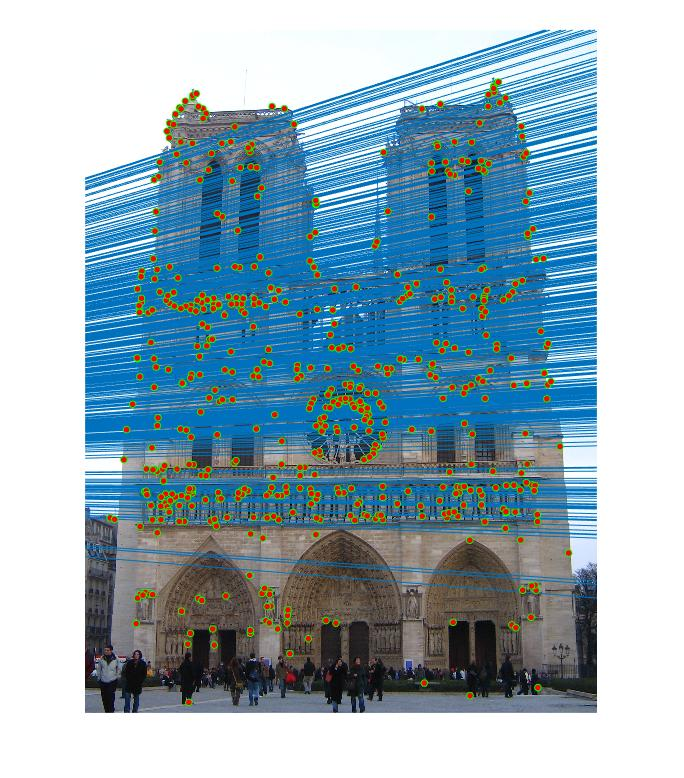
\includegraphics[scale=0.25]{notre_dame_img1_epipolar_lines.jpg}
    \caption{Image 1 epipolar lines.}
  \end{minipage}
  \hfill
  \begin{minipage}[b]{0.4\textwidth}
    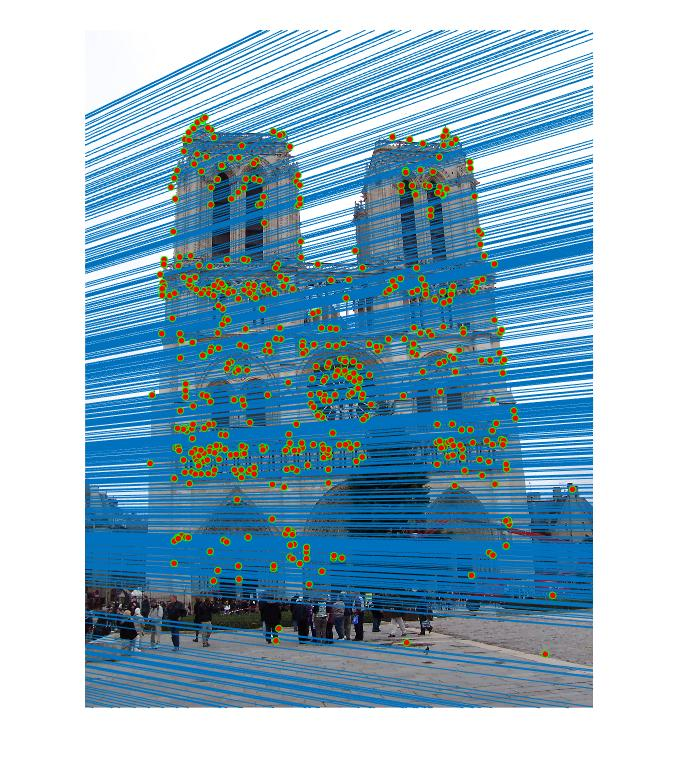
\includegraphics[scale=0.25]{notre_dame_img2_epipolar_lines.jpg}
    \caption{Image 2 epipolar lines.}
  \end{minipage}
\end{figure}
\end{center}

\begin{center}
\begin{figure}[H]
			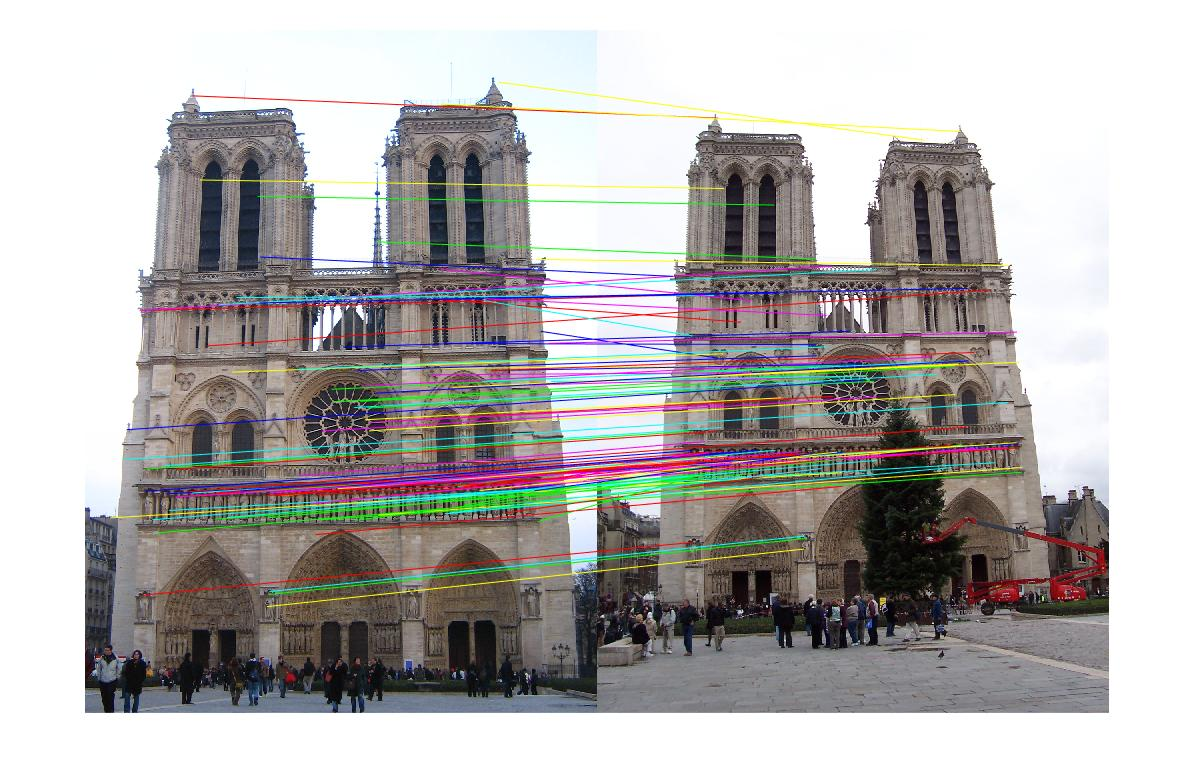
\includegraphics[scale = 0.35]{notre_dame_estimated_matches.jpg}
\caption{Notre Dame estimated matches.}
\end{figure}
\end{center}
	


		\section{Episcopal Gaudi Results}



	The results for the Episcopal Gaudi epipolar lines were not as accurate, in terms of captured inliers, as compared to the Notre Dame and Mount Rushmore results. The fundamental matrix for the Episcopal Gaudi image pair was computed using a maximum of 5000 iterations, a minimum of 40 inliers, and an error tolerance of $\epsilon = 1$.

The results for the Episcopal Gaudi image pair resulted in fairly accurate matches, however a few spurrious matches remain. To counter this, more iterations of RANSAC could be used to try a larger number of possible estimates and the error tolerance could be decreased to attempt to force more accurate matches. Decreasing the error tolerance may also result in fewer inliers, producing fewer matches in the output. 



\begin{center}
\begin{figure}[H]
  \centering
  \begin{minipage}[b]{0.4\textwidth}
    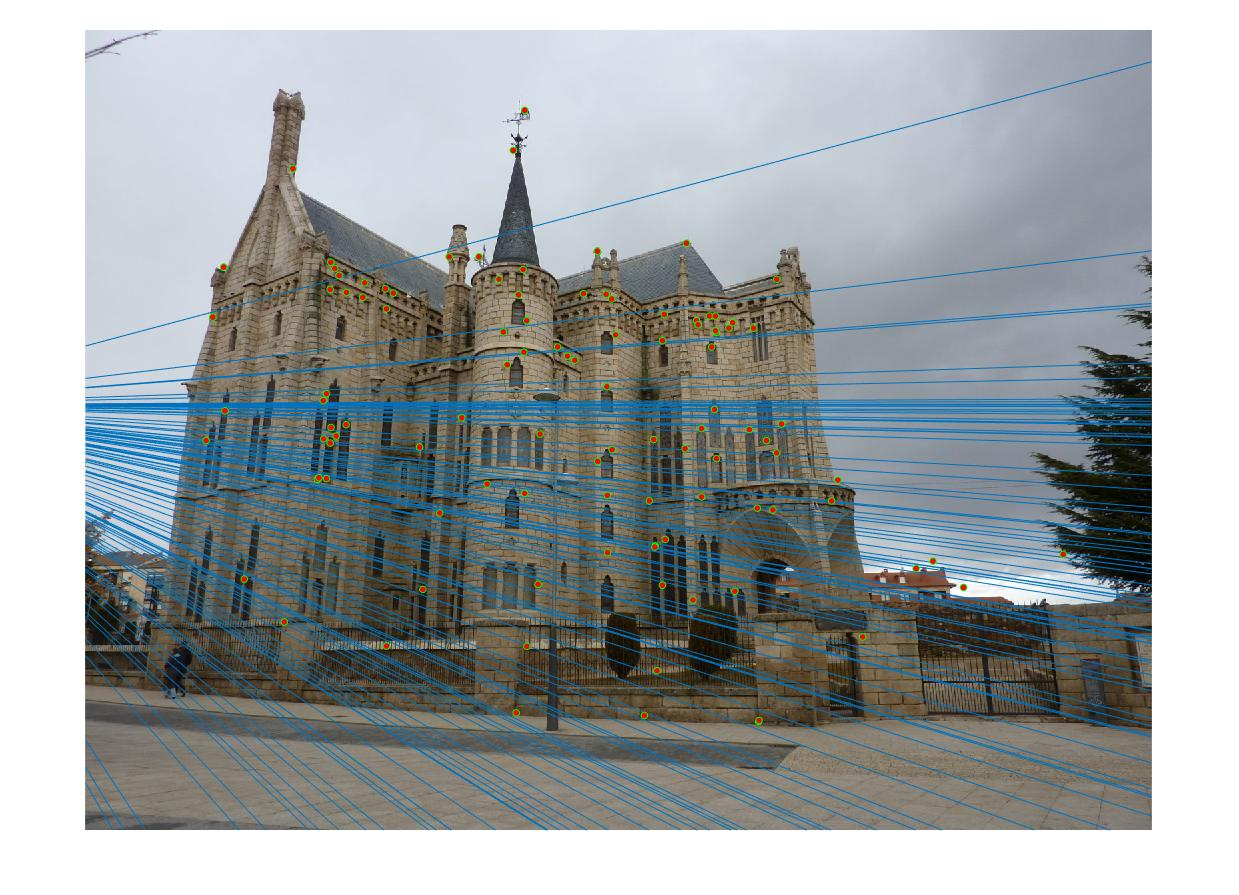
\includegraphics[scale=0.2]{episcopal_gaudi_img1_epipolar_lines.jpg}
    \caption{Image 1 epipolar lines.}
  \end{minipage}
  \hfill
  \begin{minipage}[b]{0.4\textwidth}
    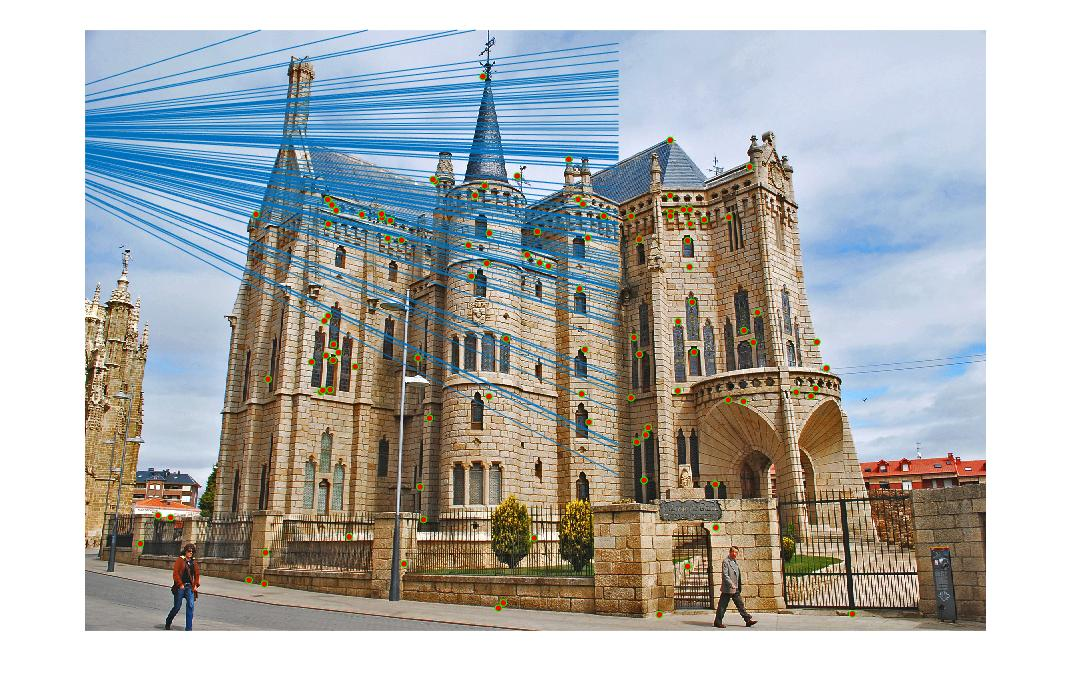
\includegraphics[scale=0.2]{episcopal_gaudi_img2_epipolar_lines.jpg}
    \caption{Image 2 epipolar lines.}
  \end{minipage}
\end{figure}
\end{center}


\begin{center}
\begin{figure}[H]
			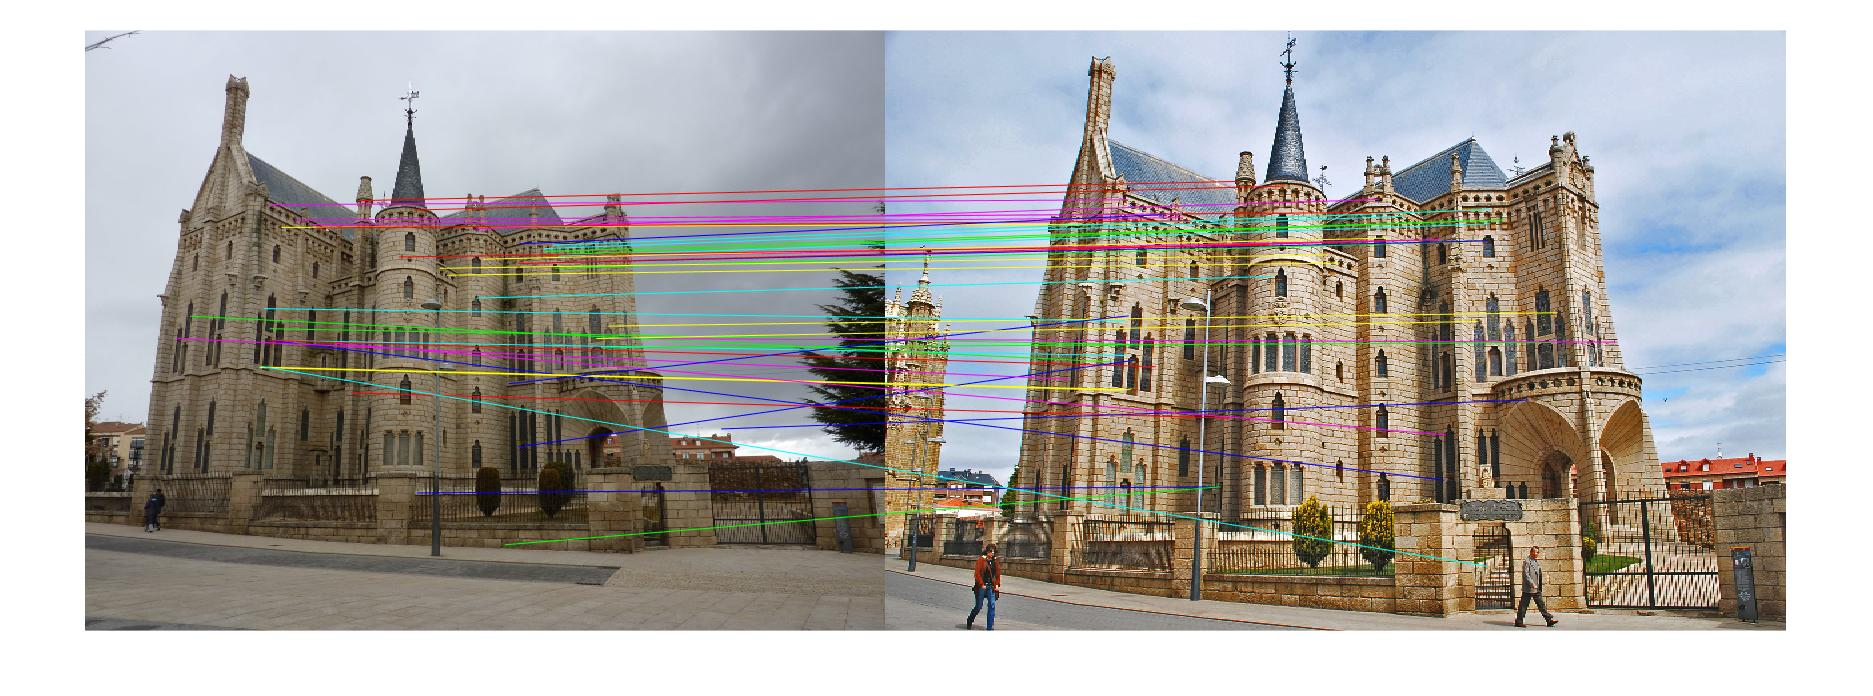
\includegraphics[scale = 0.2125]{episcopal_gaudi_estimated_matches.jpg}
\caption{Episcopal Gaudi estimated matches.}
\end{figure}
\end{center}




		\section{Mount Rushmore Results}

The fundamental matrix for the Mount Rushmore image pair was computed with RANSAC using a maximum of 5000 iterations, a minimum of 300 matches, and an error tolerance of $\epsilon = 0.1$. An immediate problem is that the provided set of matches only contains 245 match pairs, meaning that the algorithm will always take 5000 iterations before terminating. Nonetheless, the results for the Mount Rushmore image pair appeared to be the most accurate.

In particular, the matches for the Mount Rushmore image pair contain few spurrious matches. It is believed that since the algorithm completed 5000 iterations with a relatively low error tolerance, a fairly accurate set of inliers were found, resulting a good estimation of the fundamental matrix.



\begin{center}
\begin{figure}[H]
  \centering
  \begin{minipage}[b]{0.4\textwidth}
    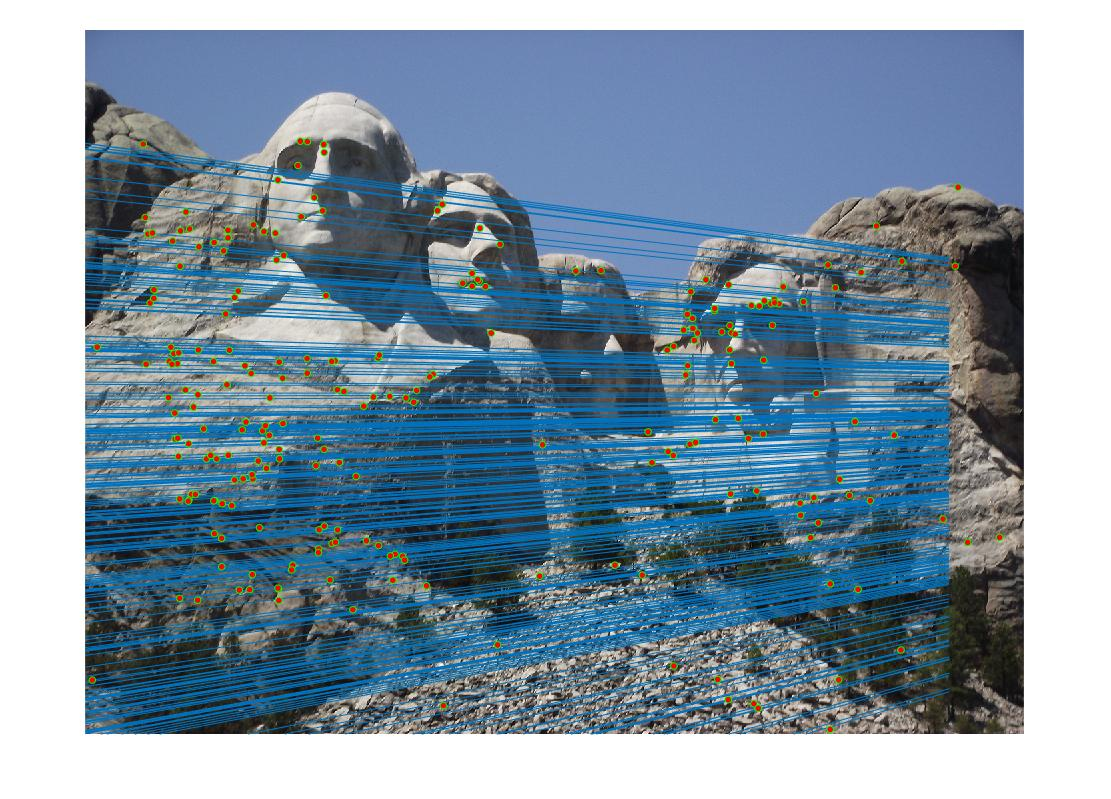
\includegraphics[scale=0.2]{mount_rushmore_img1_epipolar_lines.jpg}
    \caption{Image 1 epipolar lines.}
  \end{minipage}
  \hfill
  \begin{minipage}[b]{0.4\textwidth}
    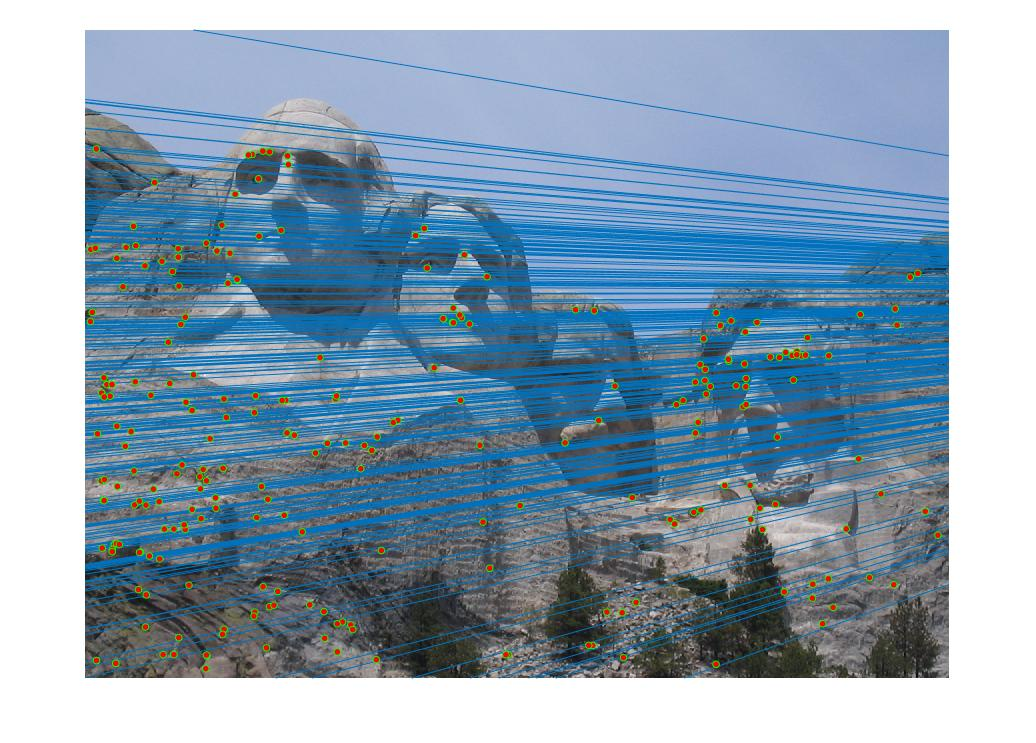
\includegraphics[scale=0.2]{mount_rushmore_img2_epipolar_lines.jpg}
    \caption{Image 2 epipolar lines.}
  \end{minipage}
\end{figure}
\end{center}

\begin{center}
\begin{figure}[H]
			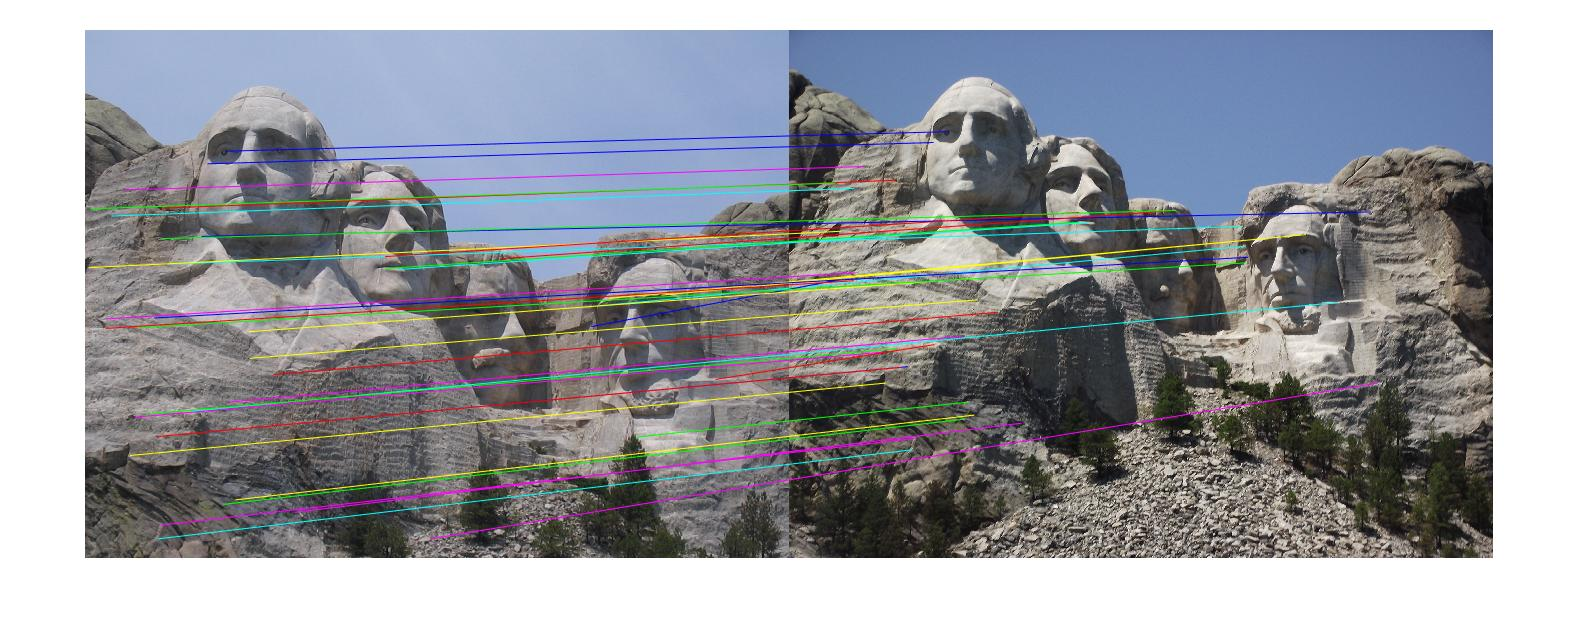
\includegraphics[scale = 0.25]{mount_rushmore_estimated_matches.jpg}
\caption{Mount Rushmore estimated matches.}
\end{figure}
\end{center}

	\section{Remarks}
	Each of the requested outputs are contained within the source code directory, estimations of the camera intrinsic matrices are also included. 
		A notable issue that arose during the implementation was the speed of the RANSAC algorithm. Specifically, the problem of speed occurs in the subroutine in which the pairwise distances between each point and epipolar line are computed. This function requires $\mathcal{O}(n^{2})$ comparisons FOR EACH iteration of the RANSAC algorithm, requiring RANSAC to have a total worst case execution time proportional to $\mathcal{O}(mn^{2})$ where $n$ is equivalent to the number of matches and $m$ is equivalent to the number of RANSAC iterations. As a consequence, parameter optimization was less than ideal. It was later discovered that the algorithm primarily had difficulties with the Notre Dame matches as there were a rather large number, but performed quite well on the Episcopal Gaudi and Mount Rushmore match sets with fewer total matches.

		Additionaly, finding the correct RQ decomposition proved to be challengin when attempting to estimate the intrinsic camera matrix (and rotation matrix). I was not able to spend more time understanding how exactly the RQ decomposition algorithm functions, however I included my results for these items in the code.
		Helper code for drawing the matches, drawing the epipolar lines, and for computing the RQ decomposition were utilized from outside sources with the references included in each function.


\end{document}